\documentclass[a4paper]{article}
\usepackage[margin=1.0in]{geometry}
\usepackage{amsmath,amssymb,bm}
\usepackage{enumitem}
\usepackage{graphicx,float}

\title{cs224n Assignment \#2: word2vec}
\date{}
\author{}

\begin{document}

\begin{center}
    \section*{cs224n Assignment \#2: word2vec}
\end{center}
\medskip

% \maketitle

\subsection*{1. Understanding word2vec}
    \begin{enumerate}[label=(\alph*)]

        % (a)
        \item Since the true empirical distribution $\bm{y}$ has a distribution such that 
        \[
            y_w = \left.
            \begin{cases}
                1, & \text{for } w = o \\
                0, & \text{elsewhere ,} 
            \end{cases}
            \right.
        \]
        \begin{flalign*}
            \text{cross-entropy loss}&=-\sum _{w\in V}y_{w}\log( \hat{y}_{w}) \\ 
            &=-y_{o}\log ( \hat{y}_{o}) -\sum _{\substack{w\in V \\ w \neq o}}y_{w}\log( \hat{y}_{w})\\ 
            &=-y_{o}\log ( \hat{y}_{o}) =-\log ( \hat{y}_{o}) \\
            &= -\log P(O=o|C-c) = \bm{J}_\text{naive-softmax} &
        \end{flalign*}

        % (b)
        \item Since $\bm{J}_\text{naive-softmax} = - \log ( \hat{y}_{o}) 
        = - \log \dfrac{\exp(\bm{u}_{o}^{\mathsf{T}}\bm{v}_{c})}{\sum _{w\in V}\exp(\bm{u}^{T}_{w}\bm{v}_{c})}
        = - \bm{u}_{o}^{\mathsf{T}}\bm{v}_{c} + \log \sum _{w\in V}\exp(\bm{u}_{w}^{\mathsf{T}}\bm{v}_{c}) $, \\
        \begin{flalign*}
            \dfrac{\partial }{\partial \bm{v}_{c}}\bm{J}
            &= \dfrac{\partial }{\partial \bm{v}_{c}} (-\bm{u}_{o}^{\mathsf{T}}\bm{v}_{c})
             + \dfrac{\partial }{\partial \bm{v}_{c}}\log \sum _{w\in V}\exp(\bm{u}_{w}^{\mathsf{T}}\bm{v}_{c}) \\
            &= - \bm{u}_{o}
            + \dfrac{\sum _{w\in V}\bm{u}_{w}\exp(\bm{u}_{w}^{\mathsf{T}}\bm{v}_{c})}
            {\sum _{w\in V}\exp(\bm{u}_{w}^{\mathsf{T}}\bm{v}_{c})} 
            = - \bm{u}_{o} + \sum _{w\in V} \bm{u}_{w} \hat{y}_{w} \\
            & = \bm{U}(\hat{\bm{y}}-\bm{y}) &
        \end{flalign*}
        
        % (c)
        \item From above, $\bm{J}_\text{naive-softmax} = - \log ( \hat{y}_{o}) 
        = - \bm{u}_{o}^{\mathsf{T}}\bm{v}_{c} + \log \sum _{w\in V}\exp(\bm{u}_{w}^{\mathsf{T}}\bm{v}_{c}) $. \\
        \begin{flalign*}
            \therefore \dfrac{\partial }{\partial \bm{u}_{w}}\bm{J}
            &= \dfrac{\partial }{\partial \bm{u}_{w}} (-\bm{u}_{o}^{\mathsf{T}}\bm{v}_{c})
             + \dfrac{\partial }{\partial \bm{u}_{w}}\log \sum _{w\in V}\exp(\bm{u}_{w}^{\mathsf{T}}\bm{v}_{c}) \\
            &= \left.
                \begin{cases}
                    \begin{alignedat}{4}
                    & - \bm{v}_{c}
                    + \dfrac{\exp(\bm{u}_{w}^{\mathsf{T}}\bm{v}_{c})\bm{v}_{c}}
                    {\sum _{w\in V}\exp(\bm{u}_{w}^{\mathsf{T}}\bm{v}_{c})} 
                    && = - \bm{v}_{c} + \hat{y}_{w}\bm{v}_{c} 
                    && = (\hat{y}_{w} - y_{w}) \bm{v}_{c}, 
                    && \text{ for } w = o \text{ since }y_{w} = 1\text{ at }w=o\\
                    & \dfrac{\exp(\bm{u}_{w}^{\mathsf{T}}\bm{v}_{c})\bm{v}_{c}}
                    {\sum _{w\in V}\exp(\bm{u}_{w}^{\mathsf{T}}\bm{v}_{c})} 
                    && {}
                    && = \hat{y}_{w}\bm{v}_{c},
                    && \text{ elsewhere} 
                    \end{alignedat}
                \end{cases}
                \right.\\
            & = \bm{v}_{c}(\hat{\bm{y}}-\bm{y})^{\mathsf{T}} &
        \end{flalign*}

        % (d)
        \item $\bm{\sigma}(\bm{x}) = \dfrac{1}{1+\exp(-\bm{x})}$
        \begin{flalign*}
            \therefore \dfrac{\partial }{\partial \bm{x}}\bm{\sigma}(\bm{x})
            &= - \dfrac{-\exp(-\bm{x})}{(1+\exp(-\bm{x}))^2} = \dfrac{1}{1+\exp(-\bm{x})} \cdot \dfrac{\exp(-\bm{x})}{1+\exp(-\bm{x})} \\
            &= \dfrac{1}{1+\exp(-\bm{x})} \cdot (1-\dfrac{1}{1+\exp(-\bm{x})}) = \bm{\sigma}(\bm{x})(1-\bm{\sigma}(\bm{x})) &
        \end{flalign*} 
        and, we can easily get $\dfrac{\bm{\sigma}'(\bm{x})}{\bm{\sigma}(\bm{x})}=1-\bm{\sigma}(\bm{x})$.

        % (e)        
        \item $\bm{J}_\text{neg-sample} = - \log (\sigma(\bm{u}_{o}^{\mathsf{T}}\bm{v}_{c})) - \sum_{k=1}^{K}\log (\sigma(-\bm{u}_{k}^{\mathsf{T}}\bm{v}_{c}))$
        \begin{flalign*}
            \therefore \dfrac{\partial }{\partial \bm{v}_{c}}\bm{J}
            &= - \dfrac{\partial }{\partial \bm{v}_{c}} \log (\sigma(\bm{u}_{o}^{\mathsf{T}}\bm{v}_{c})) 
             - \dfrac{\partial }{\partial \bm{v}_{c}} \sum_{k=1}^{K}\log (\sigma(-\bm{u}_{k}^{\mathsf{T}}\bm{v}_{c}))
            = - \dfrac{\sigma'(\bm{u}_{o}^{\mathsf{T}}\bm{v}_{c})}{\sigma(\bm{u}_{o}^{\mathsf{T}}\bm{v}_{c})}
            - \sum_{k=1}^{K} \dfrac{\sigma'(-\bm{u}_{k}^{\mathsf{T}}\bm{v}_{c})}{\sigma(-\bm{u}_{k}^{\mathsf{T}}\bm{v}_{c})} \\
            &= - \bm{u}_{o}(1-\sigma(\bm{u}_{o}^{\mathsf{T}}\bm{v}_{c})) - \sum_{k=1}^{K}-\bm{u}_{k}(1-\sigma(-\bm{u}_{k}^{\mathsf{T}}\bm{v}_{c})) \\
            &= \bm{u}_{o}(\sigma(\bm{u}_{o}^{\mathsf{T}}\bm{v}_{c})-1) + \sum_{k=1}^{K}\bm{u}_{k}\sigma(\bm{u}_{k}^{\mathsf{T}}\bm{v}_{c}) \\
            \dfrac{\partial }{\partial \bm{u}_{o}}\bm{J}
            &= - \dfrac{\partial }{\partial \bm{u}_{o}} \log (\sigma(\bm{u}_{o}^{\mathsf{T}}\bm{v}_{c})) 
             - \dfrac{\partial }{\partial \bm{u}_{o}} \sum_{k=1}^{K}\log (\sigma(-\bm{u}_{k}^{\mathsf{T}}\bm{v}_{c}))
            = - \dfrac{\sigma'(\bm{u}_{o}^{\mathsf{T}}\bm{v}_{c})}{\sigma(\bm{u}_{o}^{\mathsf{T}}\bm{v}_{c})}
            - \sum_{k=1}^{K} \dfrac{\sigma'(-\bm{u}_{k}^{\mathsf{T}}\bm{v}_{c})}{\sigma(-\bm{u}_{k}^{\mathsf{T}}\bm{v}_{c})} \\
            &= - \bm{v}_{c}(1-\sigma(\bm{u}_{o}^{\mathsf{T}}\bm{v}_{c})) = \bm{v}_{c}(\sigma(\bm{u}_{o}^{\mathsf{T}}\bm{v}_{c})-1) \\
            \dfrac{\partial }{\partial \bm{u}_{k}}\bm{J}
            &= - \dfrac{\partial }{\partial \bm{u}_{k}} \log (\sigma(\bm{u}_{o}^{\mathsf{T}}\bm{v}_{c})) 
             - \dfrac{\partial }{\partial \bm{u}_{k}} \sum_{k=1}^{K}\log (\sigma(-\bm{u}_{k}^{\mathsf{T}}\bm{v}_{c}))
            = - \dfrac{\sigma'(\bm{u}_{o}^{\mathsf{T}}\bm{v}_{c})}{\sigma(\bm{u}_{o}^{\mathsf{T}}\bm{v}_{c})}
            - \sum_{k=1}^{K} \dfrac{\sigma'(-\bm{u}_{k}^{\mathsf{T}}\bm{v}_{c})}{\sigma(-\bm{u}_{k}^{\mathsf{T}}\bm{v}_{c})} \\
            &= - \sum_{k=1}^{K}-\bm{v}_{c}(1-\sigma(-\bm{u}_{k}^{\mathsf{T}}\bm{v}_{c})) = \sum_{k=1}^{K}\bm{v}_{c}(1-\sigma(-\bm{u}_{k}^{\mathsf{T}}\bm{v}_{c})) 
            = \sum_{k=1}^{K}\bm{v}_{c}\sigma(\bm{u}_{k}^{\mathsf{T}}\bm{v}_{c}) &            
        \end{flalign*} 
        Negative sampling is more efficient because it doesn't need to use all words in vocabulary set to compute the loss but only the fraction of vocabulary set which are used in sampling.

        % (f)
        \item $\bm{J}_\text{skip-gram} = \sum\nolimits_{\substack{-m \leq j \leq m \\ j \neq 0}} \bm{J}(\bm{v}_{c}, w_{t+j}, \bm{U})$ when $\bm{J}(\bm{v}_{c}, w_{t+j}, \bm{U})$ is either $\bm{J}_\text{naive-softmax}$ or $\bm{J}_\text{neg-sample}$
        \begin{flalign*}
            \therefore \dfrac{\partial }{\partial \bm{U}}\bm{J}_\text{skip-gram}
            &= \sum_{\substack{-m \leq j \leq m \\ j \neq 0}} \dfrac{\partial }{\partial \bm{U}}\bm{J}(\bm{v}_{c}, w_{t+j}, \bm{U}) \\
            \dfrac{\partial }{\partial \bm{v}_{c}}\bm{J}_\text{skip-gram} 
            &= \sum_{\substack{-m \leq j \leq m \\ j \neq 0}} \dfrac{\partial }{\partial \bm{v}_{c}}\bm{J}(\bm{v}_{c}, w_{t+j}, \bm{U}) \\
            \dfrac{\partial }{\partial \bm{v}_{w}}\bm{J}_\text{skip-gram} 
            &= 0 \text{ for } w \neq c&
        \end{flalign*}
    \end{enumerate}

\subsection*{2. Implementing word2vec}
    \begin{enumerate}[label=(\alph*)]
        \setcounter{enumi}{2}
        \item Some similar words are very close i.e. (amazing, wonderful, great), (woman, female) as expected. 

        But some opposite words are also very close in the figure i.e. (female, man), (enjoyable, annoying).

        Also, we can find some analogies i.e (female : male :: queen : king) in the figure.
        \begin{figure}[h]
            \centering
            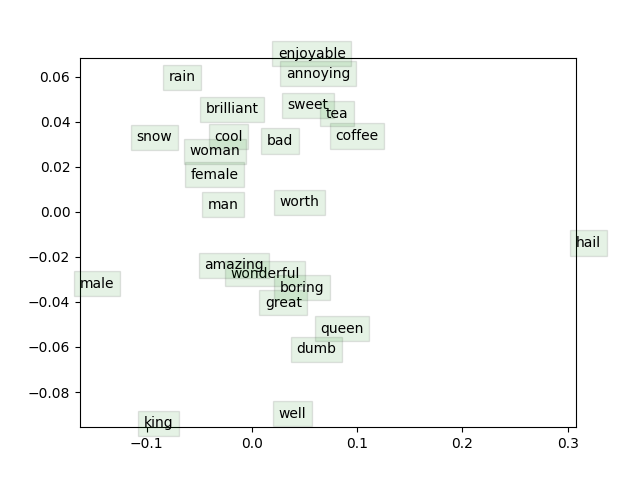
\includegraphics[width=0.4\textwidth]{word_vectors.png}
            \caption{Show time! word vectors}
            \label{fig:word_vectors}
        \end{figure}
    \end{enumerate}
\end{document}